
\documentclass[oneside,a4paper]{book}

\usepackage{pdfpages}
%\pagestyle{headings}


%=============================================================================

\usepackage{amsthm}
\usepackage{xspace}
\usepackage{float}
\usepackage{ifthen}
\usepackage{amsbsy}
\usepackage{amssymb}
\usepackage{balance}
\usepackage{booktabs}
\usepackage{graphicx}
\usepackage{rotating}
\usepackage{multirow}
\usepackage{needspace}
\usepackage{microtype}
\usepackage{bold-extra}
\usepackage{geometry}
\usepackage{varioref}
\usepackage{xcolor}
\usepackage{textcomp}
\usepackage{listings}
\usepackage[normalem]{ulem} %emphasize still italic
\usepackage{ucs}
\usepackage{pdflscape}
\usepackage{graphicx}
\usepackage{longtable}
\usepackage{float}
\usepackage{multirow}
\usepackage{tikz}
\usepackage{array}
\usetikzlibrary{shapes.callouts, positioning, shapes, arrows.meta, fit}


% \usepackage[utf8]{inputenc}
% \usepackage[htt]{hyphenat}
\usepackage{times}
\usepackage{url}
\usepackage{alltt}
\usepackage{amsmath}
\usepackage{xfrac}
\usepackage{subfigure}
\usepackage{appendix}
\usepackage{stmaryrd}   % for the \shortuparrow
\usepackage[utopia]{quotchap}

\usepackage{setspace}
\usepackage[numbers, sort&compress]{natbib}
\usepackage{mdwlist}        % support for better spaced lists
% allows for temporary adjustment of side margins
\usepackage{chngpage}
\usepackage[normalem]{ulem} 
\usepackage{tikz}
\usetikzlibrary{shapes, arrows.meta, positioning}

\tikzset{
  block/.style={rectangle, draw=black, fill=yellow!50, rounded corners, minimum height=1.2em, text centered, text width=3cm},
  module/.style={circle, draw=black, fill=blue!30, minimum size=2cm, text centered, align=center}, 
  orchestrator/.style={circle, draw=black, fill=black, text=white, minimum size=2.5cm, text centered},
  arrow/.style={-Stealth, thick}
}

% constants

\newcounter{qcounter}

% commands
\newcommand{\n}{$\cdot$}
\newcommand{\y}{\checkmark}
\newcommand{\subscript}[1]{$_{\textrm{\footnotesize{#1}}}$}
\newcommand{\superscript}[1]{$^{\textrm{\footnotesize{#1}}}$}
\newcommand{\vertical}[1]{\raisebox{-4em}{\begin{sideways}{#1}\end{sideways}}}

\newboolean{showedits}
\setboolean{showedits}{true} % toggle to show or hide edits
\ifthenelse{\boolean{showedits}}
{
       \newcommand{\ugh}[1]{\textcolor{red}{\uwave{#1}}} % please rephrase
       \newcommand{\ins}[1]{\textcolor{blue}{\uline{#1}}} % please insert
       \newcommand{\del}[1]{\textcolor{red}{\sout{#1}}} % please delete
       \newcommand{\chg}[2]{\textcolor{red}{\sout{#1}}{\ra}\textcolor{blue}{\uline{#2}}} % please change
}{
       \newcommand{\ugh}[1]{#1} % please rephrase
       \newcommand{\ins}[1]{#1} % please insert
       \newcommand{\del}[1]{} % please delete
       \newcommand{\chg}[2]{#2}
}


% ============================================================================
% Put edit comments in a really ugly standout display

\usepackage{xcolor}
\usepackage[normalem]{ulem}
\newcommand{\ra}{$\rightarrow$}


% comments \nb{label}{color}{text}
\newboolean{showcomments}
\setboolean{showcomments}{true}
\ifthenelse{\boolean{showcomments}}
    {\newcommand{\nb}[3]{
        {\colorbox{#2}{\bfseries\sffamily\scriptsize\textcolor{white}{#1}}}
        {\textcolor{#2}{\sf\small$\blacktriangleright$\textit{#3}$\blacktriangleleft$}}}
     \newcommand{\version}{\emph{\scriptsize$-$Id$-$}}
%	 \newcommand{\ugh}[1]{\textcolor{red}{\uwave{#1}}} % please rephrase
%	 \newcommand{\ins}[1]{\textcolor{blue}{\uline{#1}}} % please insert
%	 \newcommand{\del}[1]{\textcolor{red}{\sout{#1}}} % please delete
%	 \newcommand{\chg}[2]{\textcolor{red}{\sout{#1}}{\ra}\textcolor{blue}{\uline{#2}}} % please change
	 \newcommand{\chk}[1]{\textcolor{ForestGreen}{#1}} % changed, please check
	}
    {\newcommand{\nb}[3]{}
     \newcommand{\version}{}
	\newcommand{\chk}[1]{} % changed, please check
	}

% ============================================================================
% Make quotes be italic
\renewenvironment{quote}
    {\list{}{\rightmargin\leftmargin}%
     \item\relax\begin{it}}
    {\end{it}\endlist}

\newcommand{\ttimes}{\ensuremath{\times}}

%=============================================================================

\newcommand{\needlines}[1]{\Needspace{#1\baselineskip}}

% source code
\usepackage{xcolor}
\usepackage{textcomp}
\usepackage{listings}
\definecolor{source}{gray}{0.9}
\lstset{
	language={},
	% characters
	tabsize=3,
	upquote=true,
	escapechar={!},
	keepspaces=true,
	breaklines=false,
	alsoletter={:},
	breakautoindent=true,
	columns=fullflexible,
	showstringspaces=false,
	basicstyle=\footnotesize\ttfamily,
	% background
	frame=single,
    framerule=0pt,
	backgroundcolor=\color{source},
	% numbering
	numbersep=5pt,
	numberstyle=\tiny,
	numberfirstline=true,
	% captioning
	captionpos=b,
	numberbychapter=false,
	% formatting (html)
	moredelim=[is][\textbf]{<b>}{</b>},
	moredelim=[is][\textit]{<i>}{</i>},
	moredelim=[is][\uline]{<u>}{</u>}}
\newcommand{\ct}{\lstinline[backgroundcolor=\color{white},basicstyle=\footnotesize\ttfamily]}
\newcommand{\lct}[1]{{\small\tt #1}}


%----------------------------------------------------------------------------
% references
\newcommand{\tabref}[1]{\hyperref[{tab:#1}]{Table~\ref*{tab:#1}}}
\newcommand{\figref}[1]{\hyperref[{fig:#1}]{Figure~\ref*{fig:#1}}}
\newcommand{\secref}[1]{\hyperref[{sec:#1}]{Section~\ref*{sec:#1}}}
\newcommand{\lstref}[1]{\hyperref[{lst:#1}]{Listing~\ref*{lst:#1}}}
\newcommand{\charef}[1]{\hyperref[{cha:#1}]{Chapter~\ref*{cha:#1}}}
%----------------------------------------------------------------------------

% abbreviations
\tracingcolors 4
\setcounter{tocdepth}{3}
\setcounter{secnumdepth}{3}
\newcommand{\ie}{\emph{i.e.,}\xspace}
\newcommand{\eg}{\emph{e.g.,}\xspace}
\newcommand{\etc}{\emph{etc.}\xspace}
\newcommand{\etal}{\emph{et al.}\xspace}


\newcommand{\newevenside}{
	\ifthenelse{\isodd{\thepage}}{\newpage}{
	\newpage
        \phantom{placeholder} % doesn't appear on page
	\thispagestyle{empty} % if want no header/footer
	\newpage
	}
}

\def\stretchfactor{1}
\newcommand{\mychapter}[1]{\setstretch{1}
    \chapter{#1}\setstretch{\stretchfactor}}

%----------------------------------------------------------------------------
\newcommand{\lessSpace}{\vspace{-1em}}
\DeclareGraphicsExtensions{.pdf,.png}
\graphicspath{{images/}}
\newcommand{\fig}[4]{
	\begin{figure}[#1]
		\centering
		\includegraphics[width=#2\textwidth]{#3}
		\lessSpace
		\caption{\label{fig:#3}#4}
	\end{figure}}

% ===========================================================================


\newcommand{\thesistitle}{Evaluating the Effects of Experiencing a Mixed Reality Simulation of Symptoms of Schizophrenia on Empathy in Medical Students}
\newcommand{\thesisauthor}{Ann Kiener}
\newcommand{\thesisleiter}{Prof. Elena Mugellini}
\newcommand{\thesisasst}{Prof. Denis Lalanne}
\newcommand{\thesissubtitle}{Thesis subtitle}
\newcommand{\thesisdate}{\today}



% ===========================================================================

\usepackage[ colorlinks=true, urlcolor=black, linkcolor=black,
			citecolor=black, bookmarksnumbered=true, bookmarks=true,
			plainpages=false,
			pdftitle={\thesistitle}, pdfauthor={\thesisauthor},
			pdfsubject={\thesissubtitle}, pdfpagelabels]{hyperref}

\newcommand{\hrref}[2]{\hyperref}
% ===========================================================================
% ===========================================================================


% D O C U M E N T
% % % % % % % % % % % % % % % % % % % % % % % % % % % % % % % % % %
\begin{document}

% T I T L E
% % % % % % % % % % % % % % % % % % % % % % % % % % % % % % % % % %
\begin{titlepage}  
  \begin{center}  
  
  \begin{figure}[t]  
  \vspace*{-2cm}        % to move header logo at the top 
  \center{
\includegraphics[scale=0.2]{logos/MSc_quer.png}}
  \vspace{0.4in}     
  \end{figure}

    \thispagestyle{empty}
    
    {\bfseries\Huge \thesistitle \par}
    %\Large \vspace{0.1in} \thesissubtitle \par}

    \vspace{0.3in} 
    \LARGE{\textbf{Master Thesis} \\}
    \vspace{0.4in}

    {\Large \thesisauthor}
    
    \vspace{0.3in}
    {\Large University of Bern \par}
%    {\Large Philosophisch-naturwissenschaftlichen Fakult\"{a}t \\
%            der Universit\"{a}t Bern \par}
    \vspace{0.3in}
    {\Large \emph{supervised by} \par}
    {\Large \thesisleiter \par}
    {\Large \thesisasst \par}
    \vfill
    {\Large \thesisdate \par}
    
  

  \vspace{0.9in}
 
  % === Logos ==============================================     
  \begin{figure}[htp]
    \centering
    
\includegraphics[scale=0.30]{logos/UNI_Bern.png}\hfill
    
\includegraphics[scale=0.30]{logos/UNI_Neuenburg.png}\hfill
    
\includegraphics[scale=0.80]{logos/UNI_Fribourg.png}
  \end{figure}
  % === // Logos ===========================================    


  \end{center}

\end{titlepage}


% A B S T R A C T
% % % % % % % % % % % % % % % % % % % % % % % % % % % % % % % % % %
\chapter*{\centering Abstract}
\begin{quotation}
\noindent 
Abstract (max. 1 page)

Name of the Supervisor, Group, Institute, University, Supervisor

Name of the Assistant, Group, Institute, University, Assistant
\end{quotation}
\clearpage


% C O N T E N T S 
% % % % % % % % % % % % % % % % % % % % % % % % % % % % % % % % % % % % % % % %
\tableofcontents

%%%%%%%%%%%%%%%%%%%%%%%%%%%%%%%%%%
%%%% NEW CHAPTER %%%%%%%%%%%%%%%%%%%%%
%%%%%%%%%%%%%%%%%%%%%%%%%%%%%%%%%%
%\chapter{Introduction}
%\label{cha:introduction}
%
%\chapter {Related Work}
%In which we learn what have other done to address similar problems. For example, the work of Star \cite{Star89}
%
%\chapter{The Problem}
%In which we understand what the problem is in detail.
%
%\chapter {The Solution}
%In which you describe your solution.
%
%\chapter {The Validation}
%In which you show how well the solution works.
%
%\chapter {Conclusion and Future Work}
%In which we step back, have a critical look at the entire work, then conclude, and learn what lies beyond this thesis.

\chapter{Introduction}
\label{ch:introduction}

\emph{The purpose of a report is to transmit coherent information on a subject to the target readers. Reports are usually technical and should be based on verifiable facts or experiments. It is not a chronological description of your work. Obviously, the requirements of your readers (and tutors especially) must be taken into account: what information is requested, how much does the reader know already, what interests him/her? Write your report in such a way that your fellow students will be able to understand it and can put the contained information to use. Try to use short sentences to explain your work rather than long never-ending sentences.}

\subsection{Project Background}
\emph{Explain the context of your work. Motivate the relevance of your project within its context.}

\subsection{Scope of Project}
\emph{Explain the scope of your project.}
\newpage{\pagestyle{empty} \cleardoublepage}


\chapter{Background}
\label{ch:background}

Short abstract to the chapter (a quick summary of all the sections)

\begin{itemize}
\item Describe the prior work relevant to the topic
\item The work should be grouped meaningfully (according to the conventions in the topic) so that it is easier to get an overview.
\item The number of references should be $\ge 20$ for a BSc thesis and $\ge 40$ for an MSc thesis.
\item Introduce relevant notation and background knowledge if needed (possibly in a separate chapter)
\end{itemize}

\section{Immersive Learning Experiences}

\section{Schizophrenia Simulations}

\section{Empathy}

\section{Prior Work}
Here we describe concrete prior work that includes all three sections > immersive learning experiences, schizophrenia simulations, and empathy.


\newpage{\pagestyle{empty} \cleardoublepage}

\chapter{Prior Work}
\label{ch:priorwork}

Here we describe concrete prior work that includes all three sections > immersive learning experiences, schizophrenia simulations, and empathy.


\newpage{\pagestyle{empty} \cleardoublepage}

\chapter{Name of the approach/Name of the problem}
\label{ch:method}

\emph{This chapter can also be split into multiple chapters depending on the case.}

Short abstract to the chapter (a quick summary of all the sections)

\begin{itemize}
\item Describe the problem to be solved formally and use illustrations to present it
\item Describe the ideas of the approach used to solve the problem
\end{itemize}
\newpage{\pagestyle{empty} \cleardoublepage}


\chapter{Experiments}
\label{ch:experiments}

Short abstract to the chapter (a quick summary of all the sections)

\begin{itemize}
\item Describe the list of experiments and provide the rationale (what do you want to demonstrate with these experiments?)
\item Describe all the settings needed to carry out the experiments (as if you instructed someone else to replicate them)
\item Structure the experiments meaningfully: For example, first all synthetic experiments and then all experiments on real data.
Another important section is to show Ablation studies, where one can demonstrate the effect of each component in the proposed solution.
\item Provide both quantitative (numbers, overall statistics) and qualitative (pictures, some examples) results.
\item Provide critical analysis of both quantitative and qualitative experiments: Why did something work or not work? Why better/worse?
\item Focus on critical cases: Worst errors/Best performance examples. Discuss them.
\item Do the experiments demonstrate achieving the original objective? Is the analysis making conclusions about the original objectives?
\end{itemize}
\newpage{\pagestyle{empty} \cleardoublepage}


\chapter{Conclusion}
\label{ch:conclusions}


This master thesis investigated the effectiveness of a brief Mixed Reality simulation designed to enhance both affective and cognitive empathy in medical students towards patients with schizophrenia. The aim was to explore whether immersing students in simulated symptoms, complemented by education and structured debriefing, could reshape their empathy and perceptions towards people living with this stigmatized and often misunderstod condition.

\section{Key Findings}
While the quantitative analysis of this study, using the JSE and B-PANAS, did not show statistically significant changes in empathy scores or emotional affect across the whole group, important insights were gained, even from these results. The pre-evaluation revealed that participants already possessed a relatively high baseline level of empathy, which may have limited the room for significant improvement.

\vspace{1em}

Addtionally, the qualitative findings provided evidence of meaningful cognitive and emotional engagement. Participants experiencing the simulation frequently reported strong emotional reactions, including difficulties in focusing, feelings of helplessness, and general discomfort. Crucially, many participants articulated that the experience altered their perspective on living with schizophrenia, showing increased compassion and understanding. There was also some variability in how visible users reactions were to the observing participants, which shows different nature of the immersive experience. The auditory hallucinations were often perceived as overwhelming and possibly the most impactful aspect of the simulation.


\section{Impact}
This thesis adds to the field by focusing on Mixed Reality as a tool for empathy training in medical education, addressing a gap in existing research which is more centered on Virtual Reality. MR offers unique advantages by enabling users to experience simulated symptoms while remaining in their real-world environment, therefore promoting emotional safety and relatability compared to fully immersive VR experiences which can sometimes be overwhelming.

The successful development and testing of a MR application, which can repeatedly be used, demonstrates its potential as a valuable tool for traditional learning methods in medical studies. This project highlights the capability of MR to offer an authentic yet safe experiential learning environment. In addition to that, it has the potential to prepare future healthcare providers for more compassionate and understanding interactions with patients suffering from schizophrenia or other mental health conditions. Working closely with healthcare experts and following strong ethical rules also made this project more scientifically sound and valuable for education.


\section{Outlook}

A key takeaway from this project is how crucial a good learning setup is. This includes preparing students before the simulation and, most importantly, discussing it with them afterward. Even if the measurements do not show big changes, these guided talks are crucial. They help students process the experience, understand it better, and turn their emotional reactions into empathy. This also helps prevent increasing negative ideas or stigma or making students feel more uncomfortable.

\paragraph{Future Work}
Based on what was found, here are some ideas for future research and improvements:

\begin{itemize}
    \item \textbf{Interaction Design:} The simulation could be more engaging. Some students felt unsure how to interact with the virtual parts. Giving clearer instructions or tasks that need direct responses within the Mixed Reality environment could make it more immersive and help students participate more.
    \item \textbf{Engagement:} There should be more emphasis into ways to make the experience better for students who are watching but not wearing the headset. This could help the whole group learn and develop empathy even more.
    \item \textbf{Long-term Effects and more Participants:} Future studies should check how these MR simulations affect empathy and attitudes over a longer period. In addition, it should also include more people in these studies to see if these findings apply more widely and if one can find bigger statistical differences.
    \item \textbf{Content:} The simulation content can be improved to adjust to how each user reacts. This would help find the right balance between how intense the experience is emotionally and how safe and comfortable the person feels. This way, more people can benefit from the experience.
\end{itemize}

In short, this study successfully showed that a new Mixed Reality application can be a powerful learning tool. It helps medical students better understand and empathize with people who have schizophrenia. Even though the numbers did not show major changes in empathy, the strong emotional and mental impact, plus the benefits of MR, prove its potential. This technology could really change mental health education and lead to more caring healthcare for everyone.
\newpage{\pagestyle{empty} \cleardoublepage}


\begin{appendix}
% Include: consent form, testing day protocol, OK from CEP committee (?), link to github for code, link to simulation video, questionnaires

\chapter{JSE Items}
\section*{Appendix A: JSE Items and Classification}
\label{app:jse}

\begin{table}[H]
\centering
\begin{tabular}{p{11cm}cc}
\toprule
\textbf{JSE Item} & \textbf{Cognitive} & \textbf{Affective} \\
\midrule
1. My understanding of how my patients and their families feel does not influence medical or surgical treatment. &  & X \\
2. My patients feel better when I understand their feelings. &  & X \\
3. It is difficult for me to view things from my patients’ perspectives. & X & \\
4. I consider understanding my patients’ body language as important as verbal communication in caregiver-patient relationships. & X & \\
5. I have a good sense of humor that I think contributes to a better clinical outcome. & Ambiguous & Ambiguous \\
6. Because people are different, it is difficult for me to see things from my patients’ perspectives. & X & \\
7. I try not to pay attention to my patients’ emotions in history taking or in asking about their physical health. &  & X \\
8. Attentiveness to my patients’ personal experience does not influence treatment outcomes. &  & X \\
9. I try to imagine myself in my patients’ shoes when providing care to them. & X & \\
10. My patients value my understanding of their feelings which is therapeutic in its own right. &  & X \\
11. Patients’ illnesses can be cured only by medical or surgical treatment; therefore, emotional ties to my patients do not have a significant influence on medical or surgical outcomes. & (X) & X \\
12. Asking patients about what is happening in their personal lives is unhelpful in understanding their physical complaints. & (X) & X \\
13. I try to understand what is going on in my patients’ minds by paying attention to their non-verbal cues and body language. & X & \\
14. I believe that emotion has no place in the treatment of medical illness. &  & X \\
15. Empathy is a therapeutic skill without which success in treatment is limited. &  & X \\
16. An important component of the relationship with my patients is my understanding of their emotional status, as well as that of their families. &  & X \\
17. I try to think like my patients in order to render better care. & X & \\
18. I do not allow myself to be influenced by strong personal bonds between my patients and their family members. &  & X \\
19. I do not enjoy reading non-medical literature or the arts. & Ambiguous & Ambiguous \\
20. I believe that empathy is an important therapeutic factor in medical or surgical treatment. &  & X \\
\bottomrule
\end{tabular}
\caption{Classification of JSE Items by Empathy Dimension (Cognitive vs. Affective)}
\label{tab:jse_classification}
\end{table}


\chapter{Shortened JSE Item Set}
\label{app:jse-short}

\section*{Appendix B: Reduced Set of JSE Items and Classification}

\begin{table}[H]
    \centering
    \begin{tabular}{p{10.5cm}cc}
    \toprule
    \textbf{Selected JSE Item} & \textbf{Cognitive} & \textbf{Affective} \\
    \midrule
    2. My patients feel better when I understand their feelings. & & X \\
    3. It is difficult for me to view things from my patients’ perspectives. & X & \\
    6. Because people are different, it is difficult for me to see things from my patients’ perspectives. & X & \\
    7. I try not to pay attention to my patients’ emotions in history taking or in asking about their physical health. & & X \\
    9. I try to imagine myself in my patients’ shoes when providing care to them. & X & \\
    10. My patients value my understanding of their feelings which is therapeutic in its own right. & & X \\
    12. Asking patients about what is happening in their personal lives is unhelpful in understanding their physical complaints. & & X \\
    13. I try to understand what is going on in my patients’ minds by paying attention to their non-verbal cues and body language. & X & \\
    14. I believe that emotion has no place in the treatment of medical illness. & & X \\
    15. Empathy is a therapeutic skill without which success in treatment is limited. & & X \\
    16. An important component of the relationship with my patients is my understanding of their emotional status, as well as that of their families. & & X \\
    17. I try to think like my patients in order to render better care. & X & \\
    20. I believe that empathy is an important therapeutic factor in medical or surgical treatment. & & X \\
    \bottomrule
    \end{tabular}
    \caption{Reduced JSE item set used in this study with classification into empathy components}
    \label{tab:jse_shortened}
    \end{table}
    
\chapter{Supplementary Material}


\begin{itemize}

\item   Video Demonstration of the simulation can be found at: \url{https://drive.google.com/file/d/1_U2-2wLRUy-T8k-vho5fKDLXekrJ9qi7/view?usp=drive_link}.
\item Github repository with code and simulation files: \url{https://github.com/annkiener/mr-project}.
\item Consent form for the user study: \url{https://drive.google.com/file/d/1S64vRfOto7NqJihL469CKGBPS9jUP2t7/view?usp=drive_link}.
\item Testing day protocol: \url{https://docs.google.com/document/d/1Pfp2A3ZPfArS3Pdx0nXI2fMmpRA5jsNV/edit?usp=drive_link&ouid=110405891902671233690&rtpof=true&sd=true}.
\item Request to CEP committee: \url{https://docs.google.com/document/d/1MIGT55N6jOy2Zi5T1ZnQ841Om2AiJkE4/edit?usp=drive_link&ouid=110405891902671233690&rtpof=true&sd=true}.
\item Questionnaires used in the study:
    \begin{itemize}
        \item PRE-questionnaire: \url{https://forms.office.com/r/tGFYanrk2m}.
        \item POST-questionnaire (Group): \url{https://forms.office.com/r/2MbSDq44z9}.
        \item POST-questionnaire (Individual): \url{https://forms.office.com/r/UF0Esse6td}.

    \end{itemize}
\item Participation form: \url{https://drive.google.com/file/d/1-nNCUWIuby5HlzuaIRjFZk3ooMY_exzt/view?usp=drive_link}

\end{itemize}
\newpage{\pagestyle{empty} \cleardoublepage}
\end{appendix}

\addcontentsline{toc}{chapter}{\numberline{}List of Tables}
\listoftables

\addcontentsline{toc}{chapter}{\numberline{}List of Figures}
\listoffigures

\addcontentsline{toc}{chapter}{\numberline{}Bibliography}
\bibliographystyle{plain}
\nocite{*}
\bibliography{MSc_Thesis}

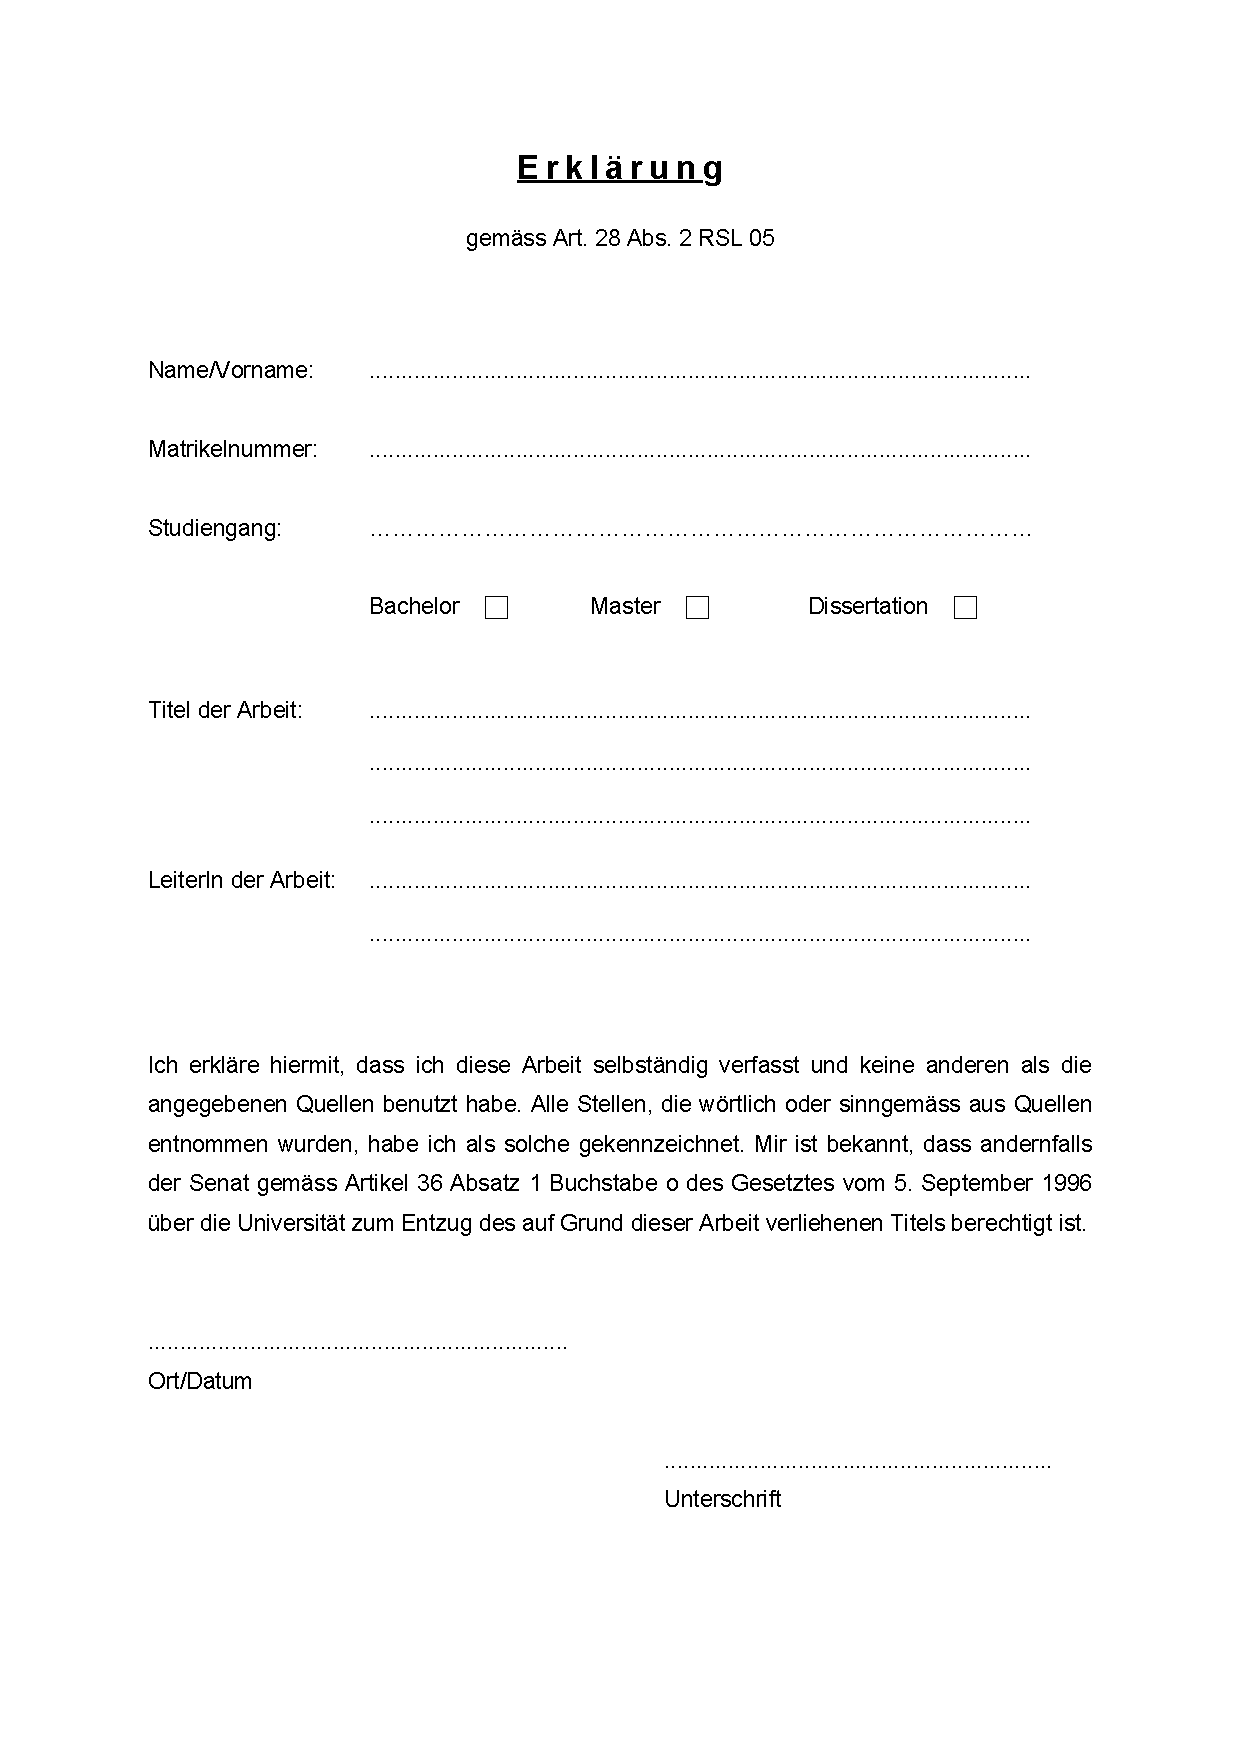
\includepdf{Erklaerung.pdf}


%END Doc
%-------------------------------------------------------

\end{document}
